% * Embedded Systems domains are diversifying
%   => rise of non-experts using embedded systems
%   => IoT innovators / SMEs building new product
%   => Educators and Students
\section{Introduction}
\label{sec:intro}

Recent years have witnessed expansive growth in the popularity and ubiquity of embedded systems. This growth can be primarily attributed to the emergence of new application domains ranging from wearables, to home automation, industrial automation, and smart grids - a phenomenon broadly referred to as the Internet of Things (IoT). As the IoT continues to grow, it has become more pervasive - far beyond the realm of domain experts and into the everyday lives of the public. This has led to growth in non-expert developers actively creating software for embedded systems. Small to medium sized business now create new products through \emph{rapid prototyping} of embedded devices. Hobbyist \emph{makers} create novel technical projects to inspire themselves and society. And now, more than ever before, \emph{educators} are making extensive use of \emph{physical computing} devices as a direct means to teach and inspire a generation of students - and to prepare them for a society where IoT will be the norm. These new developers all share a common characteristic - \emph{they are not professional software developers}~\cite{dougherty2012maker,bruce2015make,maksimovic2014raspberry}.

To drive this point home, in 2015 a consortium of industry and academic partners came together to develop the BBC micro:bit - an embedded device designed specifically for education. One million of these devices were delivered to UK school children in 2016. The micro:bit is a highly capable IoT device containing a 32 bit ARM Cortex processor, integrated light level, temperature, acceleration and magnetic sensors, touch sensitive inputs and USB and 2.4GHz Radio communications.

\begin{figure}[t]
    \centering
    \includegraphics[width=.49\columnwidth] {images/microbit-space.jpg}
    \includegraphics[width=.49\columnwidth]{images/bloodhound.jpg}
    \setlength{\belowcaptionskip}{-10pt}
    \caption{\label{fig:projects} Example projects undertaken within education: Rishworth School sent a micro:bit to space~\cite{microbit79:online} (left); The micro:bit placed in a custom-built rocket car for telemetry~\cite{microbit73:online, microsoft:online} (right).}
    \vspace{-5pt}
\end{figure}

Figure~\ref{fig:projects} highlights two example educational projects based on the BBC micro:bit. The first is a data gathering experiment, where multiple sensor data were recorded to non-volatile memory as the device was launched into near space (32.5km altitude), along with an externally interfaced camera and GPS unit. The second highlights a live data telemetry application, where acceleration data was streamed in real-time via Bluetooth Low Energy to enable the profiling of chemical-rocket powered model vehicles. These projects are highly sophisticated and were undertaken by high school educators and their students.

We introduce an open source~\footnote{
MakeCode is open source at \url{https://github.com/microsoft/pxt}; CODAL is open source at
\url{https://github.com/lancaster-university/codal}.} platform for embedded devices such as the micro:bit that enables the development of embedded applications by non-expert programmers. This platform consists of two major components: Microsoft MakeCode (\url{https://makecode.com}), a web app that consists of a beginner IDE for embedded
systems; CODAL, an efficient component-oriented C++ runtime
providing high-level programming abstractions.

In the remainder of the introduction, we present the major design challenges in
bringing embedded systems into education, briefly describe the
architecture of our solution, and give an overview of the
paper and our results.

\subsection{Design Challenges}
\label{sec:DesignChallenges}
Enabling novice programmers to successfully develop embedded applications is a non-trivial task. Throughout our research we have identified a number of design challenges that we address through MakeCode and CODAL.

\paragraph{High Level Languages:}
Programming languages for microcontroller units (MCUs) have not kept pace with advances in hardware. Despite active research in the field, the C/C++ languages remain the standard for embedded systems: they provide a familiar imperative programming model, with compilers that produce highly efficient code, and enable low level access to hardware features when necessary. The Arduino project (\url{www.arduino.cc})~\cite{buildingArduino2014}, started in 2003, and ARM's Mbed platform (\url{www.mbed.org})~\cite{ARMmbed} both rely heavily on a C/C++ programming model. However, the limitations of using C/C++ as an application programming language for inexperienced developers are well understood~\cite{blikstein2013gears}. \emph{To address this, higher level languages such as JavaScript, Python, and even visual programming languages are required}.

\paragraph{Zero Installation Architecture:}
The development environment for existing embedded systems typically requires the installation of code editors, custom device drivers, compiler toolchains, and even additional programming hardware (such as a JLink programmer). For many, particularly in the field of education, this presents a high adoption barrier as in many schools, custom hardware and software is simply not permitted by policy and/or access to the necessary technical support is not present. \emph{An effective solution must therefore provide a fully transparent, platform agnostic, zero installation experience to developing embedded software}.

\begin{table}[t]
    \centering
    \begin{tabular}{|l|r|r|r|r|r|r|}
    \hline
                           &          &              & \bf{Word}  & \bf{CPU} &            \\
    \bf{Device}            & \bf{RAM} & \bf{Flash}   & \bf{Size}  & \bf{Speed} & \bf{CPU}  \\ \hline
    Uno            & 2 kB       & 32 kB      & 8          & 16MHz & AVR       \\ \hline
    micro:bit          & 16 kB      & 256 kB     & 32         & 16MHz & Cortex     \\ \hline
    CPX           & 32 kB      & 256 kB     & 32         & 48MHz & Cortex    \\ \hline
    PC             & 16 GB      & 1 TB       & 64         & 3GHz & Intel      \\ \hline
    \end{tabular}
    \setlength{\textfloatsep}{-10pt}
    \caption{\label{table:devices}Example microcontroller devices in relationship to a typical PC. Device abbreviations: Uno (Arduino Uno), micro:bit (BBC micro:bit), CPX (Adafruit Circuit Playground Express); PC (Personal Computer).}
    \vspace{-20pt}
\end{table}

\paragraph{Optimization for Code Efficiency:}
The projects of Figure~\ref{fig:projects} are enabled by small, highly resource-limited programmable MCUs, which may have as little as a few kilobytes of RAM and FLASH memory.
Table~\ref{table:devices} compares the core capabilities of the class of MCU-based devices typically used in the education domain to a typical PC. Note that these devices have a \emph{proportionally} large amount of processing power, relative to their storage. Consider the BBC micro:bit vs. a typical PC: the micro:bit has about 100 times less CPU power, but 10\textsuperscript{6} times less RAM, and 10\textsuperscript{6} times less storage. \emph{A language/runtime should therefore not only seek to provide high code density and spatial efficiency, but actively trade off temporal for spatial efficiency where possible}.

\paragraph{Asynchronous and Concurrent Programming:}
It is already well understood that novice programmers benefit from event-based programming paradigms~\cite{maloney2008programming,maloney2010scratch,turbak2014events}. This is increasingly relevant for embedded systems due to the typically asynchronous nature of their hardware. MCUs still follow Moore's law,
but this additional capacity is not typically invested in speeding
up processors. Instead, more independent peripherals (such as Bluetooth/WiFi radio modules, audio inputs/output processors, etc.) are integrated onto the same package as the CPU as a \emph{system-on-chip}. Such peripherals often operate independently of the main CPU. \emph{An effective language/runtime should directly support an asynchronous interaction model designed to cooperate with the independent nature of peripherals while remaining highly intuitive to the programmer}.

\paragraph{Intuitive and Extensible APIs:}
Intuitive APIs and programming models are required to support novice users, yet it is equally important that these APIs remain complete enough to realise the ambitious projects that may be undertaken as students advance: simplification via the reduction of functionality is not a valid approach.
%TBALL: this sentence seems out of place - I couldn't really figure out how to make it fit.
%Also, embedded systems are becoming increasingly component based through wired and %wireless interfaces such as I2C, Bluetooth Mesh, IEEE 802.15.4.
\emph{An effective solution must provide APIs that are consistent, easy to understand/uses, and progressive, to address the growing capabilities of the programmer.}

\subsection{Architecture}

\begin{figure}[t]
    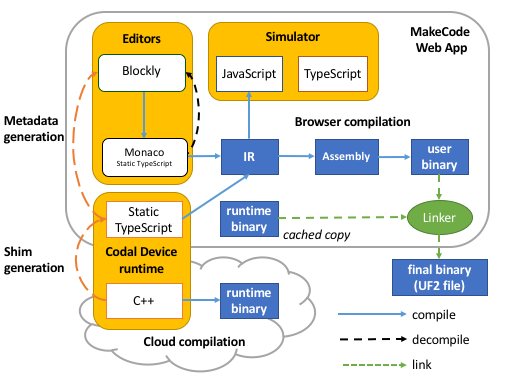
\includegraphics[width=\columnwidth]{images/arch-diagram.png}
    \setlength{\belowcaptionskip}{-10pt}
    \caption{\label{fig:makecode}The \MC and \CO Architecture}
\end{figure}

Figure~\ref{fig:makecode} illustrates the architecture of our platform.
The \MC web app is the primary entry point for the end-user. \MC supports
the simplified programming of MCUs via editors for visual blocks and textual JavaScript/TypeScript~\footnote{\url{http://typescriptlang.org}} languages .
CODAL, a component-oriented, event-driven, fiber-based C++ runtime environment that bridges the semantic gap between the higher-level languages (such
as TypeScript) and the hardware (bottom-left of the Figure). 
Enabling the flashing of the microcontroller is \UFN,
a new file format and bootloader for simplified transfer of binaries to the device over USB (bottom-right).

\MC can be accessed from any modern web browser and cached locally for \emph{entirely offline use}. The \MC web app incorporates the open source Blockly~\footnote{\url{https://github.com/google/blockly}} and Monaco~\footnote{\url{https://github.com/Microsoft/monaco-editor}} editors (upper-left), an in-browser device simulator (upper-right) for testing programs before transferring them to the physical device, as well as \emph{in-browser compilation} of TypeScript to machine code and linking against the pre-compiled
CODAL C++ runtime (lower-left).

\MC devices appear as USB pen drives when plugged into a computer, thanks to UF2. After a user has finished developing a program, the compiled binary is ``downloaded'' locally to the user's computer (lower-right) and then transferred (flashed) to the MCU by a simple file copy operation. This works out-of-the-box on any OS with built-in support for US pen drives (MacOS, Windows, Linux,ChromeOS).

\subsection{Overview}

The remainder of the paper describes the design, implementation, and evaluation of MakeCode (Section~\ref{sec:makecode}), the CODAL C++ runtime (Section~\ref{sec:codal}), and the UF2 bootloader (Section~\ref{sec:uf2}). Section~\ref{sec:evaluate} shows that together these technologies enable simplified programming while maintaining a relatively high degree of temporal and spatial efficiency. We demonstrate up to 50x better performance than other state-of-the-art implementations, in some cases nearing the performance of native C++. MakeCode has been live since the fall of 2016, at first supporting just the micro:bit, but now supporting many more devices, most of which are based on CODAL. Section~\ref{sec:related} discusses related work and Section~\ref{sec:conclude} concludes the paper.

% Our platform was deployed about a year ago at \url{www.makecode.com} and sees daily use by thousands of users.

% * Derive Requirements

% => Modern IoT Hardware
%     => Low cost
%     => 32 bit processor rich, ram poor MCUs
%     => Async h/ware

% => Universality

%   => Modern High level Langaguges
%     => Blocks
%     => Typescript
%     => C++
%     => Low barrier to entry
%     => Without sacrificing capability
%       => Temporal Efficiency
%       => Spacial Efficiency
%     => Async (HL languages are Async and the hardware is moving that way)
%     => First class Event support

%   => Modern Toolchains
%     => Universal Web based UI
%     => Driver free wired/wireless device integration

% * Paper Overview
% - background
%    - examples of awesomeness in the classroom, breaks the mould, not just blinking an LED
%    - scale
%    - non-trivial, engineering.
% - architecture
%    - makecode
%       - under the compiler section, mention no VM
%    - codal
%      - codal is not an RTOS
%    - uf2
% - eval
% - R/W
% - conclusions


% The emergence of a new breed of computer